\section{Method}

%%%%%%%%%%%%%%%%%%%%%%%%%%%%%%%%%%%%%%%%%%%%%%%%%%%%%%%%%%%%%%%%%%%%
% General diffusion models
%%%%%%%%%%%%%%%%%%%%%%%%%%%%%%%%%%%%%%%%%%%%%%%%%%%%%%%%%%%%%%%%%%%%
\subsection{Diffusion Models}
\label{sec:diffusion_models}
The diffusion framework that we use is defined theoretically as follows \cite{ddpm,improved_diffusion,EDGE}. Given $x_0 \sim p(x_0)$ from some data distribution, diffusion is a Markov noising process over latent variables $x_t, t=1,...,T$. The process of adding noise (the 'forward noising process') is defined through the distributions
\begin{equation}
    \begin{aligned}
        q(x_t|x_{t-1}) &:= \mathcal{N}(\sqrt{1-\beta_t} x_{t-1}, \beta_t \mathbf{I}) \\
        q(x_T | x_0) &:= \prod_{t=1}^T q(x_t | x_{t-1}) \\
    \end{aligned}
\end{equation}
where with a well chosen variance schedule $\beta_1, ..., \beta_T$ and a large T, we approximate a standard normal distribution as as we approach $t=T$. This entails that the first latent variable $x_T$ is approximately gaussian noise. The 'reverse noising process' is unknown without the full data distribution, which we don't have access to, hence we approximate it using some parametrized function
\begin{equation}
    \label{eq:reverse_noising_mean_variance}
    p_{\theta}(x_{t-1} | x_t) = \mathcal{N}(\mu_{\theta}(x_t, t), \Sigma_{\theta}(x_t, t))
\end{equation}

The whole process can be visualized in \figref{fig:diffusion_process} borrowed from the DDPM paper \cite{ddpm}.

\begin{figure}[!ht]
    \centering
    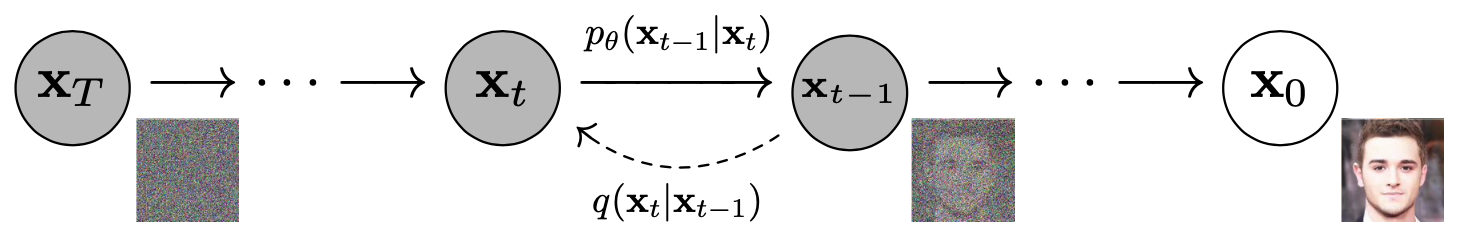
\includegraphics[width=0.75\textwidth]{Figures/diffusion/diffusion_process.png}
    \caption{Diffusion Process}
    \label{fig:diffusion_process}
\end{figure}

We find with $p$ and $q$ that this system forms a VAE that can be trained through the Variational Lower Bound (VLB) \cite{kingma2022_VAE}.

In practice however we note some modification to this definition to ease our implementation and to improve performance.
Firstly we note that the forward noising process can be written as
\begin{equation}
    \label{eq:direct_noising_latents}
    q(x_t|x_0) \sim \mathcal{N}(\sqrt{\bar{\alpha_t}}x_0, (1-\bar{\alpha_t})\mathbf{I})
\end{equation}
with $\bar{\alpha_t} = \prod_{s=1}^t \alpha_s$ and $\alpha_t = 1 - \beta_t$. This is simply a mixing of the data with gaussian noise according to a monotonically decreasing schedule $\bar{\alpha_t}$ and allows us to sample any latent at any timestep directly from the clean signal, which will aid our training procedure. We note that we take the following definition for the $\bar{\alpha_t}$ schedule (rather than defining the $\beta$ schedule), as in \cite{improved_diffusion},
\begin{equation}
    \begin{aligned}
    \bar{\alpha_t} &= \frac{f(t)}{f(0)} \\
    f(t) &= \cos \left( \frac{t/T + s}{1 + s} \cdot \frac{\pi}{2} \right)
    \end{aligned}
\end{equation}
with a small offset $s$ (we take $s=0.008$ \cite{improved_diffusion}) to avoid $\beta_t$ from being too small near $t=0$ which can reduce performance, according to the authors.

We also use a simplified reverse noising process, where rather than predicting the mean and variance of the noise for a single step as indicated in \eqref{eq:reverse_noising_mean_variance}, we directly try to predict the denoised signal \cite{ramesh2022hierarchical},
\begin{equation}
    \label{eq:denoised_signal_prediction}
    \hat{x}_{\theta}(x_t, t) \approx x_0 \\
\end{equation}
which, alongside the choice of a fixed rather than learned variance as in \cite{ddpm}, allows us to describe the denoising process as follow, where a tractable expression is provided by Bayes Theorem \cite{improved_diffusion},
\begin{equation}
    \label{eq:direct_prediction_denoising}
    \begin{aligned}
    p_{\theta}(x_{t-1} | x_t) &= q(x_{t-1} | x_t, \hat{x}_{\theta}(x_t, t))  \\
    &= \mathcal{N}(\mu_{\theta}(x_t, t), \tilde{\beta}_t I)
    \end{aligned}
\end{equation}
with 
\begin{equation}
    \label{eq:direct_prediction_denoising_details}
    \begin{aligned}
    \tilde{\beta}_t &= \frac{1 - \bar{\alpha}_{t-1}}{1 - \bar{\alpha}_t} \beta_t \\
    \mu_{\theta}(x_t, t) &= \frac{\sqrt{\bar{\alpha}_{t-1}}\beta_t}{1-\bar{\alpha}_t}\hat{x}_{\theta}(x_t, t) + \frac{\sqrt{\alpha}_t(1-\bar{\alpha}_{t-1})}{1-\bar{\alpha}_t}x_t
    \end{aligned}
\end{equation}

This direct prediction of the denoised signal allows us to use a the simplified MSE objective \cite{ddpm,ramesh2022hierarchical} during training
\begin{equation}
    \label{eq:simple_loss}
    \mathcal{L}_{simple} = \mathbb{E}_{x_0,t}\left[ \| x_0 - \hat{x}_{\theta}(x_t, t) \|_2^2 \right]
\end{equation}
which can still be interpreted as a form of Variational Lower Bound without the variance terms.

The essential idea of training such a model is to randomly sample a timestep, noise a signal back to this timestep with \eqref{eq:direct_noising_latents}, predict the denoised signal with \eqref{eq:denoised_signal_prediction}, and perform a backward step on the loss described in \eqref{eq:simple_loss} alongside some other regularisation losses that suit our problem.

The inference procedure involves sampling random gaussian noise, then iteratively predicting the denoised signal with \eqref{eq:denoised_signal_prediction} and sampling from the next timestep with \eqref{eq:direct_prediction_denoising}.

%%%%%%%%%%%%%%%%%%%%%%%%%%%%%%%%%%%%%%%%%%%%%%%%%%%%%%%%%%%%%%%%%%%%
% Our diffusion model
%%%%%%%%%%%%%%%%%%%%%%%%%%%%%%%%%%%%%%%%%%%%%%%%%%%%%%%%%%%%%%%%%%%%
\subsection{Disney Motion Diffusion (DMD)}
\label{sec:disney_motion_diffusion}
Armed with this understanding of diffusion, we define our Disney Motion Diffusion (DMD) model, strongly inspired by the work of Tevet. et. al \cite{MDM}.



\subsubsection{State Representation}
\label{sec:diffusion_state_representation}
Our state represents a motion sequence of length $N$, and includes primarily a root translation, $r \in \mathbb{R}^{N \cross 3}$, and 6d \cite{aa_6d_angles} joint orientations in body frame, $o \in \mathbb{R}^{N \cross 6}$. The state can be extended with some optional extras, depending on the data, of foot ground contacts $b \in \mathbb{R}^{N \cross 1}$, and explicit velocities for the root translation and joint orientations. Again, depending on the data, we can represent the root translation, and root orientations (a subset of the joint orientations) either in world space, where each motion sequence will have a distinct starting point and starting orientation, or as what we call a 'stuck root' reference frame, where the first pose is set to the positions $(0,0)$ and identity root orientation and all subsequent poses are described with respect to this first frame, with the idea being that this formulation leads to a smaller space for the model to learn.



\subsubsection{Architecture}
We follow closely \cite{MDM} in our architecture, though without the text conditioning. We use a simple transformer \cite{vaswani2017attention} encoder as the denoising network, conditioned on the diffusion timestep so that the network can learn how much noise is present that needs removing. This is used with the as described denoising process which can be seen in \figref{fig:dmd_architecture}.

\TODO{Link to appendix with more details on the architecture choices, number of hidden layers, etc}

\begin{figure}[!ht]
    \centering
    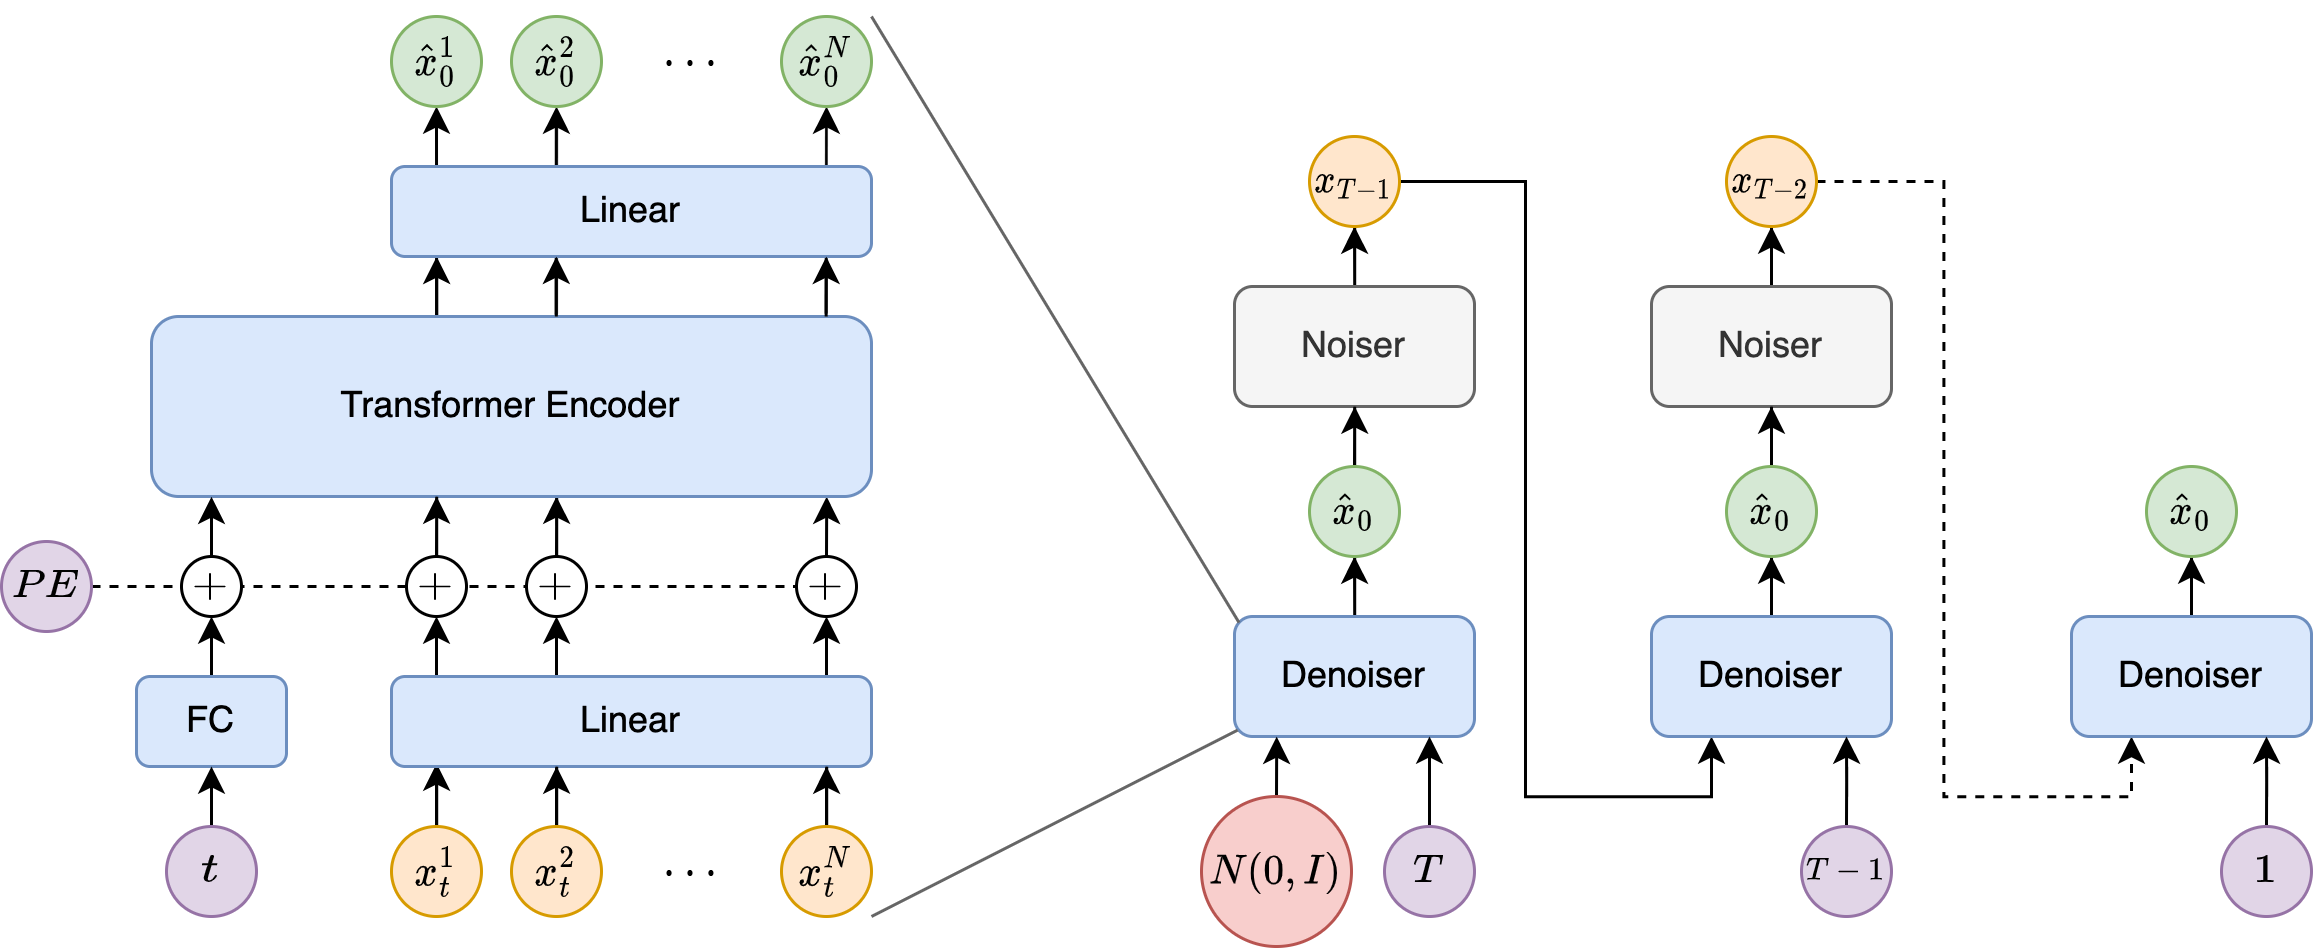
\includegraphics[width=1\textwidth]{Figures/diffusion/Network_diagram.png}
    \caption{DMD Architecture \& Denoising Process}
    \label{fig:dmd_architecture}
\end{figure}



\subsubsection{Training}
In addition to the simple MSE loss described in section \ref{sec:diffusion_models}, we can include a number of other losses to aid the training procedure.
\begin{equation}
    \begin{aligned}
        \mathcal{L}_{fk} &= \frac{1}{N} \sum_{i=1}^{N} \| x_0^{(pos)} - FK(\hat{x}_0^{(i)})  \|_2^2 \\
        \mathcal{L}_{vel} &= \frac{1}{N-1} \sum_{i=1}^{N-1} \| (x_0^{(i+1)} - x_0^{(i)}) - (\hat{x}_0^{(i+1)} - \hat{x}_0^{(i)}) \|_2^2 \\
        \mathcal{L}_{contact} &= \frac{1}{N-1} \sum_{i=1}^{N-1} \| \left( FK(\hat{x}_0^{(i+1)}) - FK(\hat{x}_0^{(i)}) \right) \cdot \hat{b}^{(i)}  \|_2^2
    \end{aligned}
\end{equation}
with $x_0^{(i)}$ representing the $i$th pose of the motion sequence $x_0$. The $\mathcal{L}_{fk}$ loss is a forward kinematics loss, i.e a loss on the positions that are calculated from the orientations through a forward kinematic function and compared to the ground truth positions that we have access to, $x_0^{(pos)}$, and which provides another mechanism by which the orientations might be adjusted, thus increasing the robustness of the predictions. The $\mathcal{L}_{vel}$ loss is a calculated velocity loss, in which the first order finite differences are used to estimate the velocities of the state (orientations and root translation only in this case), and which encourages the model to learn a smooth motion sequence. The $\mathcal{L}_{contact}$ loss is a foot contact loss, where the velocities of the ground contacting feet joints, indicated by the predicted foot contacts $\hat{b}^{(i)}$, are minimised so as to discourage foot sliding. We note that the $\mathcal{L}_{contact}$ loss is only used when the ground contacts are included in the state representation.



\subsubsection{Inpainting}
\label{sec:diffusion_method_inpainting}

An important tool in the arsenal of the diffusion model literature is that of inpainting \cite{diffusion_inpainting}. Inpainting is the process of keeping a portion of the state constant throughout the diffusion process. An example of the use of this technique would be that of changing the motion of the lower body while mainting the motion of the upper body, though there are many other use cases that are explored in more detail in \secref{sec:diffusion_experiments}. The inpainting procedure works as follows; at each denoising step we mix a portion of the latent variable state $\hat{x}_t$, indicated through the binary mask $m$, with the complementary portion of some known state $x^{(known)}$, indicated through $1-m$, 
\begin{equation}
    \hat{x}_{t} = m \odot \hat{x}_t + (1-m) \odot q(x^{(known)}|t-1)
\end{equation}
Graphically this process can be seen in \figref{fig:inpainting}. This procedure is particularly attractive at it requires no special training procedure, and can be employed readily with any diffusion model.

\begin{figure}[!ht]
    \centering
    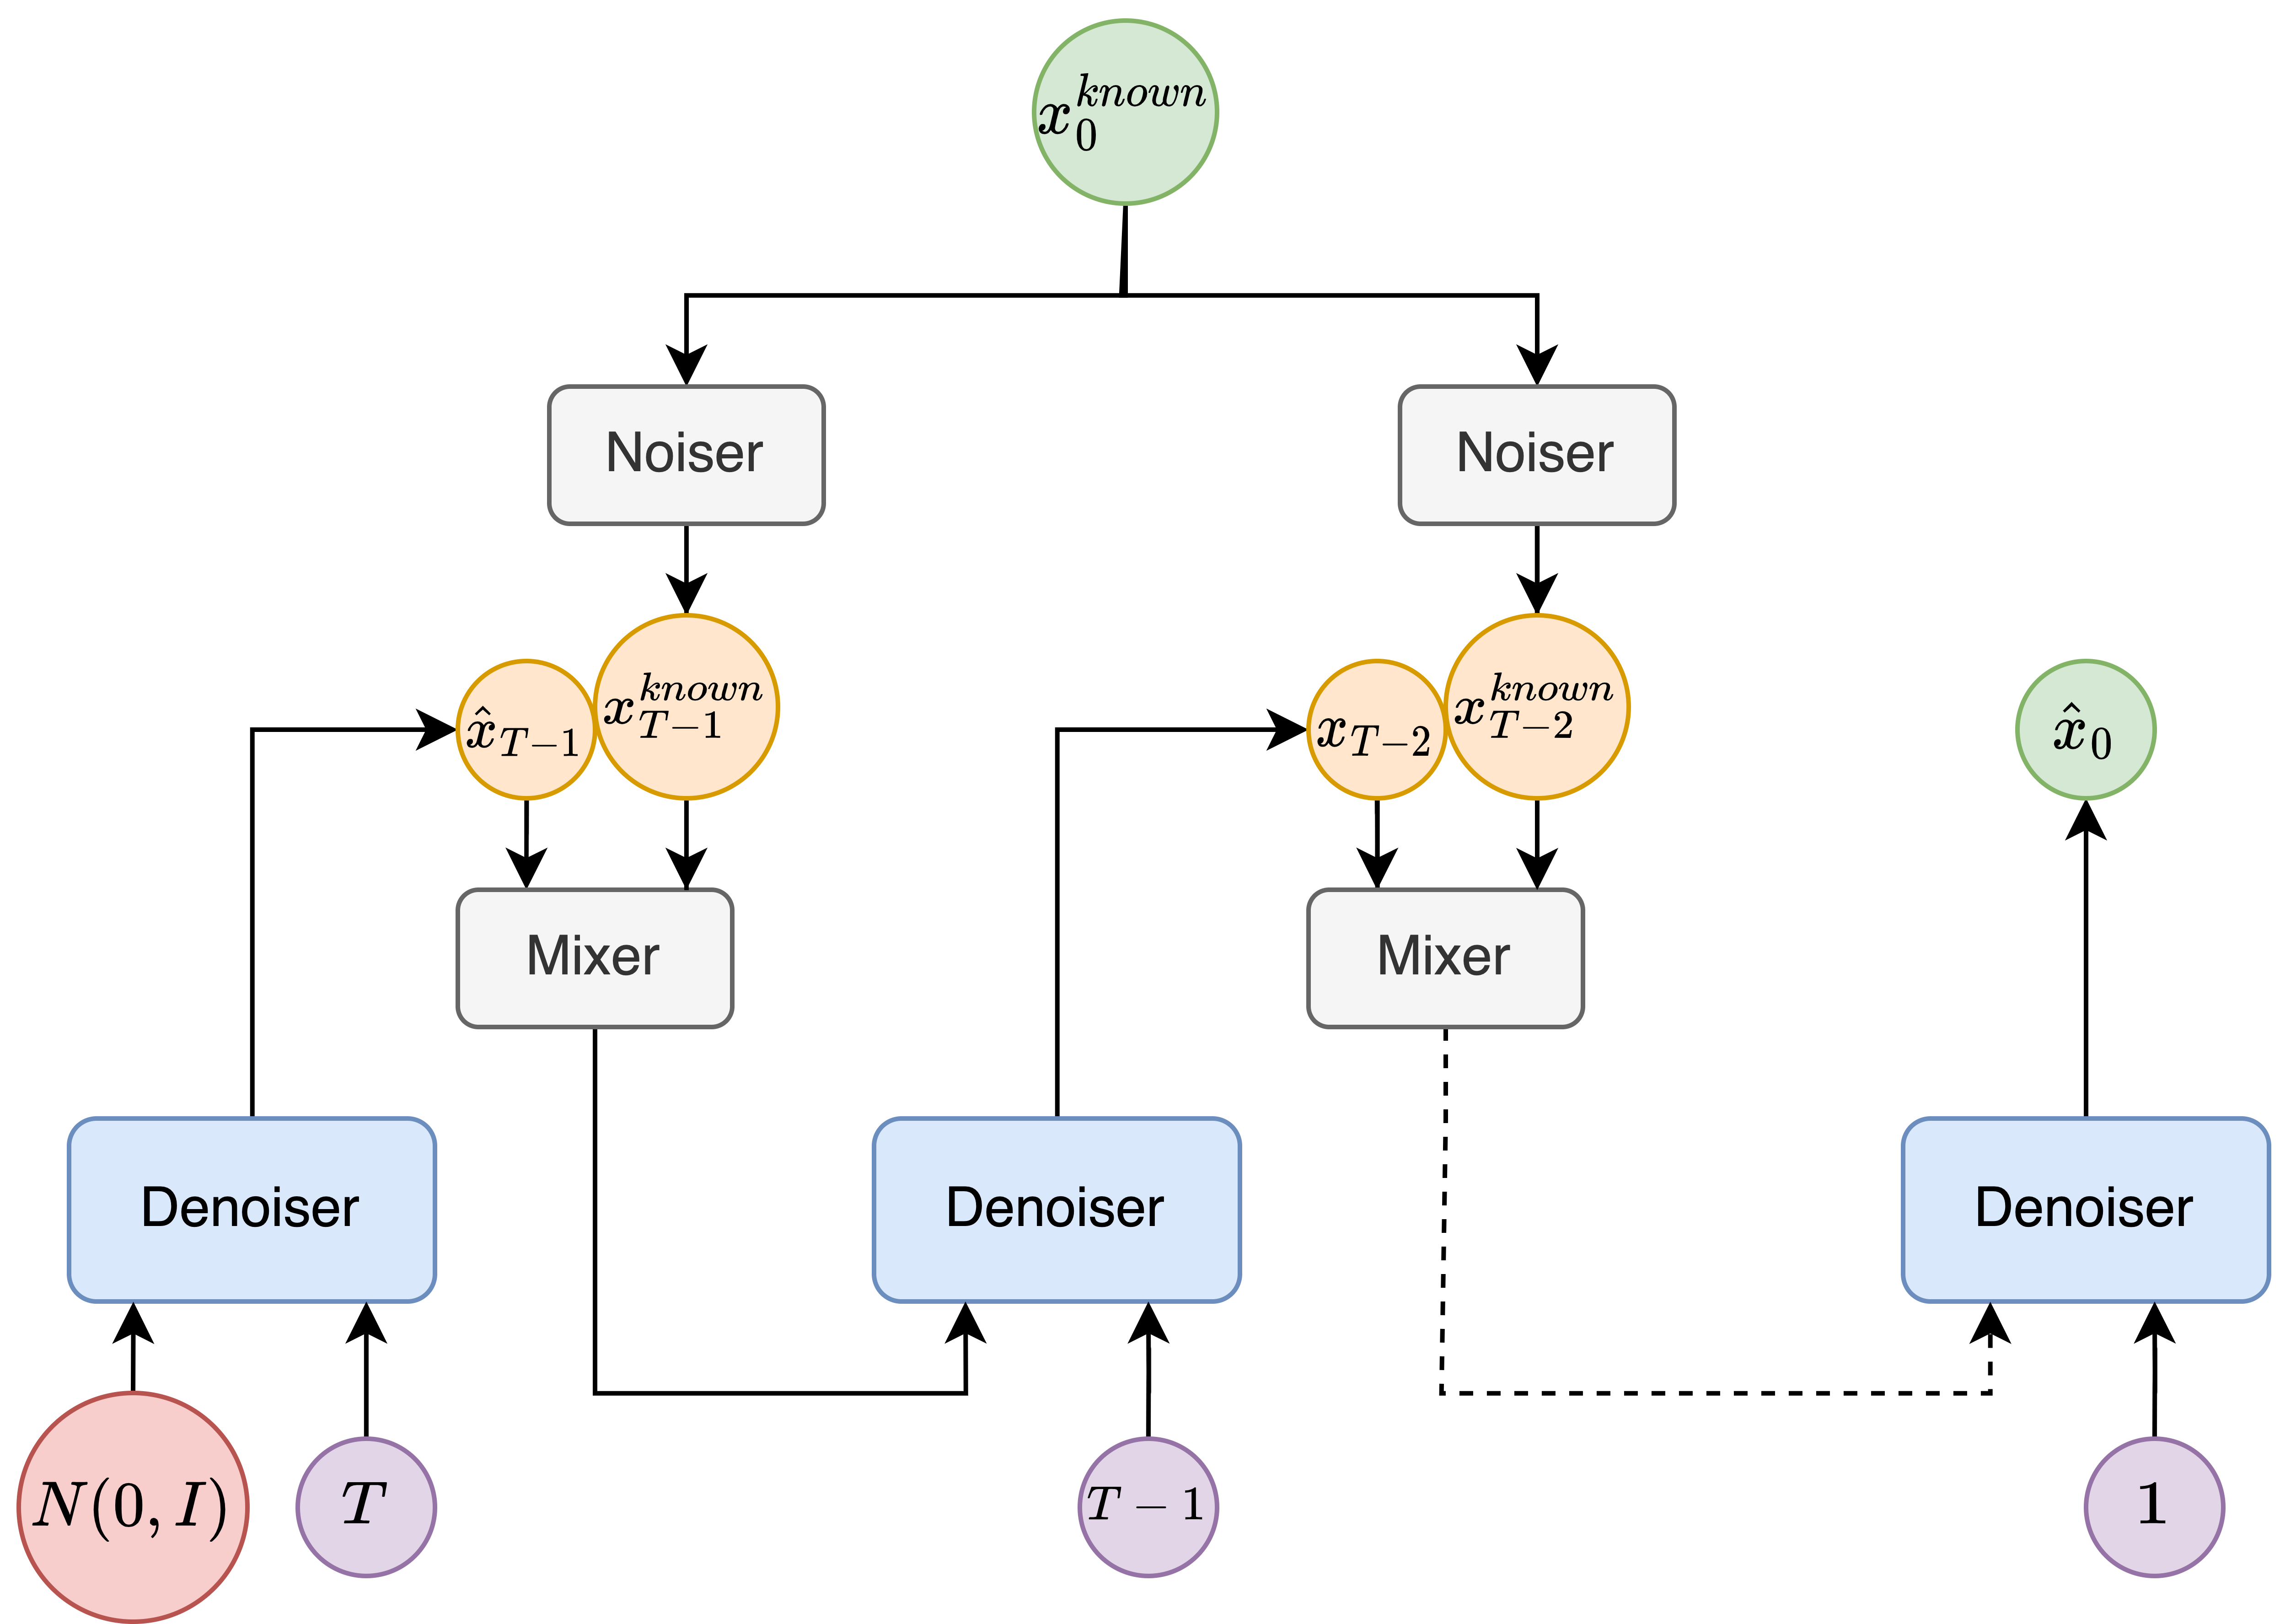
\includegraphics[width=1\textwidth]{Figures/diffusion/Inpainting.png}
    \caption{Inpainting Procedure}
    \label{fig:inpainting}
\end{figure}


\subsubsection{Data}
At Disney Research|Studios we have access to professionally capture motion capture data that encompases a wide range of possible motion for a number of subjects. In total we have \TODO{X} motion sequences, varying in length from \TODO{X} to \TODO{X} seconds long, thus in total we have \TODO{X} minutes of motion capture data. This data is normalised elementwise and retargeted to a standard skeleton. A number of motion sequences are held out for testing.

\TODO{Describe dataset 1 (fixed root, not contacts, etc) and 2 (moving root, stuck root, contacts, how to get contacts, etc.)}
